%! Author = partsjoo
%! Date = 16.04.2023


\newpage


\section{Differential privacy of query Q2}

\begin{figure}[ht]
  \begin{lstlisting}
SELECT MAX(score) (
SELECT COUNT(*) AS score FROM votes
GROUP BY candidate
) ORDERED BY score DESC LIMIT 1;
  \end{lstlisting}
  \caption{Q2: The histogram of vote counts of all candidates.}
  \label{fig:histogramQ2}
\end{figure}

\subsection{Choosing the epsilon}

Given the sensitivity $\Delta f = 1$ and the probability
of selecting the true candidate $P(T) \geq 0.9$, we want to
find the suitable $\epsilon$ value for the exponential mechanism~\cite[]{the_exponential}.
We can write the inequality for the probability of selecting a different candidate $P(C)$:

\begin{figure}[ht]
  \smaller
  \centering
  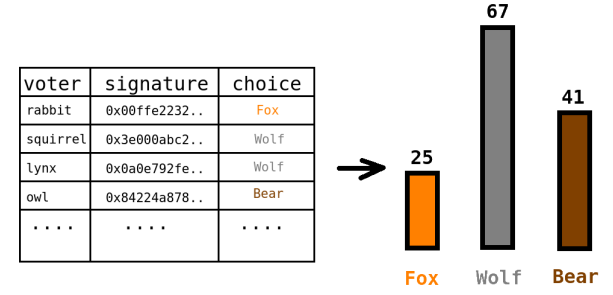
\includegraphics[width=\textwidth, keepaspectratio]{assets/fig1}
  \caption{Example vote dataset (left) and the corresponding election result (right) taken from Differential Privacy Homework}
  \label{fig:my_label5}
\end{figure}

\begin{equation}
  P(C) \leq 0.1
\end{equation}

Assuming the worst-case scenario where the difference in
score between the true candidate and the next highest candidate is 1, we can solve for $\epsilon$:

\begin{align*}
  \exp\left(\frac{\epsilon(-1)}{2}\right) &\leq 0.1 \\
  \epsilon(-1) &= 2\ln(0.1) \\
  \epsilon &\approx 4.605
\end{align*}

Therefore, the programmer should choose $\epsilon \approx 4.605$ to ensure the probability of getting the correct result is at least 0.9.

Using the computed $\epsilon \approx 4.605$ and the dataset in Figure~\ref{fig:my_label5} of the provided example (Fox -- 25, Wolf -- 67
, Bear -- 41), we
can
calculate
the
probability that the system will output the actual winner (Wolf) using the exponential mechanism. I use $Z$ to
ensure
that the probabilities of all possible outcomes sum up to 1, so thhe
probabilities for each candidate
are given by:

\begin{align*}
  P(\text{Fox}) &= \frac{\exp\left(\frac{4.605(25 - 67)}{2}\right)}{Z} \\
  P(\text{Wolf}) &= \frac{\exp\left(\frac{4.605(67 - 67)}{2}\right)}{Z} \\
  P(\text{Bear}) &= \frac{\exp\left(\frac{4.605(41 - 67)}{2}\right)}{Z}
\end{align*}

The normalization constant $Z$ is $\apporx 1.00000000000000000000000114400000101$~\cite[]{norm_Z}:

\begin{equation}
  Z = \exp\left(\frac{4.605(25 - 67)}{2}\right) + \exp\left(\frac{4.605(67 - 67)}{2}\right) + \exp\left(\frac{4.605(41 - 67)}{2}\right)
\end{equation}

The probability of selecting the true winner (Wolf) is:

\begin{equation}
  P(\text{Wolf}) = \frac{\exp\left(\frac{4.605(67 - 67)}{2}\right)}{Z} \approx 0.99997
\end{equation}

\subsection{The goodness of epsilon}

1. For the group of 10 rabbits (out of 25 votes for the Fox), we need to find the $\epsilon$-DP that is actually guaranteed for the group of
10 rabbits such that the Fox won't find sensitive information about the rabbits.
Recall from above, we computed an $\epsilon \approx 4.605$ to ensure the
probability of getting the correct result is at least 0.9.
This means that the group of 10 rabbits is
guaranteed $\epsilon$-DP with $\epsilon \approx 4.605$.
If we wanted to give the rabbits more privacy, we would need to increase the value of $\epsilon$ and increase the noise, but
then we would fall short on the 0.9 probability of getting the correct result.
So for now rabbits would have to accept their privacy being $\epsilon \approx 4.605$.

2. Let's consider the definition of $\epsilon$-differential privacy~\cite[3]{10007322}:

\begin{equation}
  \forall t, t' \in \mathcal{D}, \forall y \in \mathcal{R}, \frac{Pr[Mq(t) = y]}{Pr[Mq(t') = y]} \leq e^\epsilon
\end{equation}

where $t$ and $t'$ are neighboring datasets, $y$ is the output of the mechanism, and $Mq$ is the exponential mechanism applied to the query.

We previously obtained $\epsilon \approx 4.605$. Now, we want to show that this value of $\epsilon$ does not give any privacy guarantees for at least one output $y \in {Fox, Wolf, Bear}$.

Consider the true dataset $t$ and an arbitrary neighboring dataset $t'$ that differ by one vote, such that the vote count for the true candidate (Wolf) is decreased by one, and the vote count for one of the other candidates (Fox or Bear) is increased by one.

Given this, the probabilities for each candidate in the true dataset $t$ are:

\begin{align*}
  P_t(\text{Fox}) &= \frac{\exp\left(\frac{4.605(25 - 67)}{2}\right)}{Z_t} \
  P_t(\text{Wolf}) &= \frac{\exp\left(\frac{4.605(67 - 67)}{2}\right)}{Z_t} \
  P_t(\text{Bear}) &= \frac{\exp\left(\frac{4.605(41 - 67)}{2}\right)}{Z_t}
\end{align*}

And the probabilities for each candidate in the neighboring dataset $t'$ are:

\begin{align*}
  P_{t'}(\text{Fox}) &= \frac{\exp\left(\frac{4.605(26 - 66)}{2}\right)}{Z_{t'}} \
  P_{t'}(\text{Wolf}) &= \frac{\exp\left(\frac{4.605(66 - 66)}{2}\right)}{Z_{t'}} \
  P_{t'}(\text{Bear}) &= \frac{\exp\left(\frac{4.605(41 - 66)}{2}\right)}{Z_{t'}}
\end{align*}

Check $\epsilon$-DP condition for Fox. Since $0.00676 \leq e^{4.605}$, the condition is satisfied for $y = Fox$.
\begin{equation}
  \frac{P_t(\text{Fox})}{P_{t'}(\text{Fox})} = \frac{\exp\left(\frac{4.605(25 - 67)}{2}\right)}{\exp\left(\frac{4.605(26 - 66)}{2}\right)} \approx 0.00676
\end{equation}

Check $\epsilon$-DP condition for Wolf. Since $1 \leq e^{4.605}$, the condition is satisfied for $y = Wolf$.
\begin{equation}
  \frac{P_t(\text{Wolf})}{P_{t'}(\text{Wolf})} = \frac{\exp\left(\frac{4.605(67 - 67)}{2}\right)}{\exp\left(\frac{4.605(66 - 66)}{2}\right)} = 1
\end{equation}

Check $\epsilon$-DP condition for Bear. Since $7.389 > e^{4.605}$, the condition is not satisfied for $y = Bear$
\begin{equation}
  \frac{P_t(\text{Bear})}{P_{t'}(\text{Bear})} = \frac{\exp\left(\frac{4.605(41 - 67)}{2}\right)}{\exp\left(\frac{4.605(41 - 66)}{2}\right)} \approx 7.389
\end{equation}

This means that the previously obtained $\epsilon \approx 4.605$ does not give privacy guarantees for the output $y = Bear$.

3. When I use 10 times smaller $\epsilon$, which means that $\epsilon' = \frac{4.605}{10} \approx 0.4605$.
Let's analyze affects of this change by computing new probailityes:

\begin{align*}
  P_t(\text{Fox}) &= \frac{\exp\left(\frac{0.4605(25 - 67)}{2}\right)}{Z'_t} \
  P_t(\text{Wolf}) &= \frac{\exp\left(\frac{0.4605(67 - 67)}{2}\right)}{Z'_t} \
  P_t(\text{Bear}) &= \frac{\exp\left(\frac{0.4605(41 - 67)}{2}\right)}{Z'_t}
\end{align*}

The new normalization constant is $Z'_t \approx 1.0025783$~\cite[]{norm_Z_prim}

\begin{equation}
  Z'_t = \exp\left(\frac{0.4605(25 - 67)}{2}\right) + \exp\left(\frac{0.4605(67 - 67)}{2}\right) + \exp\left(\frac{0.4605(41 - 67)}{2}\right)
\end{equation}

The new probability of selecting the true winner (Wolf) is:

\begin{equation}
  P_t(\text{Wolf}) = \frac{\exp\left(\frac{0.4605(67 - 67)}{2}\right)}{Z'_t} \approx 0.824
\end{equation}

As we can see, the probability of getting the correct result (Wolf) is now approximately $0.824$,
which is lower than the previous probability ($\approx 0.99997$) obtained
with $\epsilon \approx 4.605$.
This reduction in accuracy is a trade-off for stronger privacy guarantees.
Even though the accuracy has decreased, a probability of $0.824$ for selecting
the true winner can still be considered reasonable in my opinion.

4. I am not entierly sure if the programmer overreacted by taking a smaller $\epsilon$.
From $\epsilon \approx 4.605$ to 10x drop into $\epsilon \approx 0.4605$ in that sense is quite a big change relative to the original value.
Even though I just concluded that change was reasonable... Reminder that Wolf had $\approx 0.824$ change with the $\epsilon \approx 0.4605$,
Fox had $\approx 0.090$(not in formula) and Bear had $\approx 0.086$(not in formula) respectivley, I think
that the
programmer should
have taken a
smaller steps
to
decide what would
be the appropriate $\epsilon$ to stop at. Having a near $8-9\%$ chance to pick the wrong candidate(Fox or Bear) in the election might just
be a
bit
too
high of a chance in my opinion. Perhaps trying different levels of privacy budgets $\epsilon$ and seeing how the
usefulness of the data vs. privacy changes in the output might give more insight into what $\epsilon$ level is appropriate.
